\documentclass[11pt]{article}

% arXiv-style single-column preprint layout
\usepackage[letterpaper,margin=1in]{geometry}
\usepackage{amsmath,amssymb}
\usepackage{booktabs}
\usepackage{microtype}
\usepackage{times}
\usepackage[T1]{fontenc}
\usepackage[utf8]{inputenc}
\usepackage{titlesec}
\usepackage{enumitem}
\usepackage[hidelinks]{hyperref}
\usepackage{url}
\Urlmuskip=0mu plus 1mu\relax  % allow URLs to break at any point
\usepackage{xcolor}
\usepackage{array}
\usepackage{pifont}
\usepackage{makecell}
\usepackage{graphicx}
\graphicspath{{figs/}}

\titleformat{\section}{\normalfont\large\bfseries}{\thesection}{0.6em}{}
\titleformat{\subsection}{\normalfont\normalsize\bfseries}{\thesubsection}{0.5em}{}
\setlength{\parskip}{0.4em}
\setlength{\parindent}{0pt}
\renewcommand{\arraystretch}{1.15}

\newcommand{\xmark}{{\color{red!70!black}\ding{55}}}

\title{\textbf{The Last Writer Wins:\\ Installing Epistemic Disposition in Multi-Agent LLM Pipelines}}
\author{Sam Bobo}
\date{Draft v0.6 --- July 2026 \quad$\vert$\quad Target: arXiv cs.CL}

\begin{document}
\sloppy  % prefer inter-word stretch over overfull boxes (arXiv-safe)
\maketitle

\begin{abstract}
\noindent
Multi-agent LLM pipelines route work through specialist models and aggregate their outputs through a synthesizer. We study \emph{disposition}---what a model chooses to emit independent of what it knows, operationalized as five epistemic behaviors, four of which proved detectable in our cases (training-cutoff disclosure, modeled-assumption flagging, jurisdictional distinguishing, and hedging; vocabulary-precision fell below detection under two independent instruments)---and ask where disposition in a pipeline comes from and whether it can be installed. Across ${\sim}1{,}300$ audited runs of a four-model ``Council of Experts'' on consumer hardware, we find: (1)~the lift usually credited to multi-agent orchestration is not a property of the topology: holding the model fixed and varying only the architecture across six designs (single-shot, flat merge, two-round debate, self-refine, prompted single model, and the council), multi-agent structure alone lifts disposition negligibly (flat merge $0.16$ vs.\ single-shot $0.14$) and a single prompted model matches the full council on magnitude ($0.50$ vs.\ $0.57$, overlapping CIs). What the council uniquely achieves is \emph{calibration}: it is the only architecture reaching substantial disposition with a clean trigger-free control ($0.00$ $[0.00,0.00]$ vs.\ the prompted model's $0.15$ $[0.08,0.22]$), because its preservation instruction is \emph{conditional} on real specialist signal; (2)~upstream installation fails robustly: prompting and supervised fine-tuning on behavior-rich exemplars produce large seat-level lifts ($\approx 2\times$, bootstrap CIs excluding baseline) that are indiscriminate---both hedge on a trigger-free control case---and that vanish from the pipeline's final output, while reference-free preference optimization installs no seat-level magnitude across three model lineages (Mistral, Llama-3, Qwen-3), invariant to a $3.2\times$ increase in preference data. Preference optimization's one real effect is subtractive and conditional: on the weakly-aligned legal seat it suppresses unwarranted hedging below baseline---a finding that survives triangulation across three instruments (pattern-based, NLI entailment, and unanimous dual LLM judges) and generalizes across objectives (ORPO and CPO), though only ORPO suppresses \emph{selectively}; the effect has no purchase on an already-aligned seat and did not replicate on a third lineage. Triangulation also caught one finding produced by the primary metric alone (an apparent hedging \emph{increase} on the finance seat) and retired it as instrument artifact; (3)~the mechanism is not sentence-level content entanglement (refuted, $r=-0.10$) but a \textbf{synthesizer register}: each aggregator model writes at its own characteristic disposition density, nearly independent of seat input---over-dense input can \emph{invert} output density---while the synthesis prompt's preservation instructions act as a \emph{graded} gain control: output density rises with the number of preservation clauses on all three synthesizers tested (Spearman $\rho=+1.00$, $+0.80$, $+0.80$; strictly monotone only on gpt-oss, with a dip at $k{=}2$ on Qwen and at $k{=}3$ on Phi-4), spanning $2$--$3\times$ on gpt-oss and Qwen and $1.3\times$ on Phi-4. The register also survives direct attack --- ORPO-training the synthesizer itself on synthesis-level pairs moves its band no more than seat training moved the seats, and heating one, two, or all three seats adds nothing at the pipeline's mouth (non-additive, $\rho=-0.80$). Weight-level training fails at every locus; \textbf{the accessible control surface is the last writer's instructions}. Practically: a pipeline's epistemic posture is governed by its last writer and that writer's instructions; upstream installation is mostly futile. The evidence base: 1{,}293 pre-registered, audited runs across three model lineages, six installation arms, and both pipeline loci (seats and the synthesizer itself), scored under three independent instruments with unanimous judge agreement on the surviving positive claim---all \$0-budget and fully reproducible on a single 32\,GB consumer machine.
\end{abstract}

\section{Introduction}
Production LLM systems increasingly take the form of pipelines: multiple models, often specialized, whose outputs are aggregated by a final model into the answer a user sees. Evaluation practice, however, remains largely single-model: we measure whether \emph{a model} hedges appropriately, discloses its limits, or labels assumptions. This paper asks what happens to those behaviors \emph{inside a pipeline}---who originates them, whether they can be installed, and whether they survive aggregation.

We distinguish two evaluation axes that are conflated in practice. \textbf{Content} is whether the right substantive material appears (measured here by per-case expert rubrics). \textbf{Disposition} is what a model chooses to emit about its own claims. Our experiments show these axes are orthogonal---the model family that wins content loses disposition and vice versa---and that pipeline disposition is governed almost entirely by the final aggregation stage.

\begin{figure}[t]
\centering

\includegraphics[width=\linewidth]{fig_schematic.pdf}
\caption{The last writer wins. Specialist seats emit disposition at densities
that vary with the installation arm (orange bars), but the synthesizer
normalizes everything to its own characteristic \emph{register band}; the
synthesis prompt's PRESERVE instructions act as a gain control on that band.
Final-output disposition (green) is nearly independent of what the seats emit
(\S\ref{sec:register}, Fig.~\ref{fig:register}).}
\label{fig:schematic}
\end{figure}

\textbf{Contributions.} (i)~A controlled comparison of six orchestration architectures with the model held fixed, isolating what multi-agent structure does and does not buy for epistemic disposition, plus a two-axis evaluation of a heterogeneous local specialist pipeline with a composite disposition metric (CDS) (\S\ref{sec:arch}). (ii)~A controlled comparison of installation mechanisms---prompting, exemplar SFT, and reference-free preference optimization (ORPO and CPO)---under pre-registered predictions, with a trigger-free control case that separates \emph{responsive} from \emph{habitual} behavior, replicated across three seats of distinct model lineage (\S\ref{sec:install}). (iii)~Identification, ablation, and stress-testing of the \textbf{synthesizer register} as the mechanism governing which installed behaviors reach the pipeline's output: it survives direct ORPO training of the synthesizer---including an on-policy, calibration-shaped, pipeline-mouth-scored retry---seat input is non-additive, and the synthesis instructions form a measured, monotone gain control (\S\ref{sec:register}). We further show the \emph{intrinsic} band is model-invariant across five models and four alignment lineages, relocating the register from a baseline emission tendency to a per-model gain coefficient on instructions (\S\ref{sec:provenance}). (iv)~A three-instrument measurement-validation protocol (pattern matching, calibrated NLI entailment, blinded pairwise LLM judges) that both confirms the surviving claims and catches a false finding produced by the primary metric (App.~\ref{app:instruments}). (v)~A fully local, \$0, consumer-hardware protocol with append-only audit logs for all 1{,}293 runs.

\section{Related work}
\textbf{Multi-agent orchestration.} Debate and role-played collaboration improve factuality and reasoning \cite{du2023,moa2024,medagents,mdagents}, and recent work compares orchestration against the strongest single model \cite{tian2025} or trains orchestrators end-to-end \cite{masorchestra}. A 2026 line now reports that well-prompted single agents match or beat multi-agent systems under matched token budgets \cite{singleagent}; our architecture comparison reproduces that negative result on a new axis (disposition \emph{magnitude}) and then identifies an axis where orchestration does pay---\emph{calibration}---which that literature does not measure. This literature measures content outcomes. The closest work on the \emph{aggregation} step, Parallel-Synthesis \cite{parallelsynth}, trains a synthesizer adapter and explicitly distills reasoning behavior from text-concatenation synthesis---an implicit acknowledgment that naive aggregation loses behavior, which our register mechanism explains and quantifies for epistemic behavior specifically. We measure what orchestration does to epistemic behavior and find an amplification effect independent of the model filling the seats.

\textbf{Specialists vs.\ generalists.} Evidence is mixed on whether small domain fine-tunes beat larger generalists in-domain \cite{trident,medftrag}. Our content results replicate the negative side (a 20B open MoE outperforms a four-specialist council $42\% \rightarrow 25$--$31\%$ on rubric coverage) and motivate the pivot: the surviving specialist value is dispositional, not informational.

\textbf{Uncertainty expression and abstention.} Verbalized uncertainty \cite{lin2022}, linguistic calibration \cite{mielke2022}, knowing-what-you-know \cite{kadavath2022}, abstention training \cite{rtuning} and recent confidence-aware abstention work \cite{icalm,bas} train and evaluate single models end-to-end. A parallel line asks whether epistemic markers \emph{faithfully} track a model's internal confidence---and finds systematic deficiencies \cite{markerfaith,rhetmiscal,markerrel}. Our contribution is orthogonal to faithfulness: we take marker \emph{emission} as the observable and ask where it originates and survives in a pipeline, not whether it is calibrated to hidden confidence. A seat's trained uncertainty behavior must survive an aggregator, and mostly does not. The closest single-model neighbor is certainty distortion \cite{certdist}:
LMs rephrasing scientific and clinical text systematically fail to preserve the
source's expressed certainty, distorting up to 75\% of outputs with a
$1.5$--$2\times$ asymmetry toward \emph{inflating} confidence, compounding
under repeated paraphrase, and only partly mitigated by prompt interventions.
A clinical benchmark reports the same failure for diagnostic uncertainty under
summarization \cite{possdef}. Both study \emph{one} model transforming text
and neither attempts to install the behavior by training. We differ on all
three axes: our object is a multi-agent pipeline where distinct specialist
models feed an aggregator; we test installation by prompting, SFT, ORPO and CPO
at both loci (and find weights move nothing); and we characterize the
aggregator's \emph{register}---a writer-specific output band nearly
independent of input, which can \emph{invert} under over-dense input rather
than merely attenuate. Their prompt-mitigation result and our gain curve
converge from different directions on the same practical conclusion, which we
regard as mutual corroboration. Two further 2026 lines make the pipeline
dimension timely: ``confidence laundering'' \cite{laundering} names, as a position, the loss of decision uncertainty at agent interfaces and argues for a latent uncertainty carrier; and a quantitative line propagates \emph{numeric} confidence estimates through multi-step agent decisions \cite{uprop}. We complement both empirically and from the opposite direction: we measure \emph{emitted linguistic disposition}, show its loss is not an interface accident but a property of the last writer (the register), and show that upstream training cannot push behavior through it.

\textbf{Register beyond epistemics.} Independent evidence for a register-like
effect comes from stylistic rewriting: \cite{voicerev} finds that LLMs revising
personal narratives shift all thirteen measured linguistic markers in the
\emph{same direction} across three frontier models---toward a more polished,
less situated register---regardless of user intent, and that voice-preserving
prompts reduce the effect magnitude by $32\%$ without changing its direction.
That is our mechanism in a different behavioral domain: a rewriter imposes its
own band, and instructions are a partial counter-lever. Their per-model effect
sizes also differ ($|d| = 0.60$, $1.29$, $1.45$), consistent with our finding
that models differ in instruction \emph{gain} rather than in baseline
emission. We differ in object (epistemic disposition, not voice), in setting
(a multi-agent pipeline, not single-stage rewriting), and in testing whether
the band can be moved by training at all---which they do not attempt.

\textbf{Preference optimization for behavior.} DPO \cite{dpo} and ORPO \cite{orpo} are standard for style/behavior shaping; DPO's length bias is documented \cite{lengthbias}, which our pair-construction controls address. Preference-data scaling is itself contested: simply adding more samples per prompt often fails to improve and can degrade downstream behavior \cite{sweetspot,air}---consistent with our dose-invariance null, which we further attribute to a downstream aggregation ceiling rather than to the optimizer. Comparisons of system-prompt steering vs.\ preference training exist for single models; we compare them \emph{through} a pipeline.

\section{Apparatus}
\textbf{Council.} Four local models via Ollama on a 32\,GB MacBook Air M5: Phi-4-14B Lead (planner + synthesizer), and three specialist seats---Llama3-Med42-8B (healthcare), Saul-7B-Instruct-v1 (legal), Qwen-Open-Finance-R-8B (finance), all Q4/Q8 GGUF. The Lead performs step-back decomposition \cite{stepback} and dispatches self-contained sub-questions; seats never see the original query (this architectural choice, not prompt strengthening, eliminated cross-domain lane bleed at sub-10B scale). The Lead then synthesizes under a structurally enforced Tensions-then-Synthesis prompt containing four PRESERVE instructions.

\textbf{Cases.} Seven three-domain scenarios: five failure-mode-targeted (synthesis stress, jurisdictional vocabulary, quantitative discipline, recency honesty, adversarial cross-domain tension) plus a matched disposition pair---case~6 (\emph{trigger-heavy}: demands all five behaviors simultaneously) and case~7 (\emph{trigger-light}: an organizational-strategy question warranting none). Case~7 is the \textbf{responsiveness gate}: any arm emitting disposition there is behaving habitually, not responsively.

\textbf{Scale.} 462 imported, audited runs (append-only JSON, one file per run, each carrying per-phase inputs/outputs/backends); all inference via Ollama on one fanless M5 MacBook Air, 32\,GB unified memory, 26.8\,GB Metal working set. Runs are nondeterministic across repeats even at temperature 0 (runtime batching); we treat repeats as seeds and report bootstrap intervals.

\textbf{Metrics.} Behavior density $=$ pattern-matched occurrences of the five behavior families (four detectable; see below) per 1{,}000 characters. $\text{CDS} = \text{density} \times \sqrt{\text{distinct behaviors}/5}$. $\text{ALR} = \text{council density} / \text{matched single-shot density}$. Seat-level density is computed on the specialist's own turn from the audit log; final density on the synthesized output. (Definitions and regexes are versioned with the code; see \S\ref{sec:limits}.) The five families are not uniformly distributed across seats: training-cutoff disclosure is universal (density $0.51$--$0.85$ on every seat), modeled-assumption flagging lives almost entirely on the finance seat ($0.25$ vs.\ $0.00$ elsewhere), hedging on healthcare and finance, jurisdictional distinguishing is thin everywhere, and vocabulary-precision is below detection ($\le 0.02$) on all three. The composite is therefore \emph{cutoff-dominated at the seat level}, and per-family claims below are tested on the seat that owns the family (App.~\ref{app:family}). At the pipeline's mouth the dominant family is a property of the \emph{synthesizer}, not of the seats, and differs across writers (\S\ref{sec:clause}).

\textbf{Installation arms} (legal seat, single-variable design, seed 42): $\text{A}'$ $=$ conversion-control baseline (identical Saul weights through our fp16$\to$GGUF$\to$Q4 pipeline); B $=$ a frozen behavior-spec addendum on the seat's system prompt (five behaviors, one example each, an explicit ``do not force it'' clause); SFT $=$ LoRA on 91 behavior-rich \emph{chosen} responses; ORPO $=$ LoRA reference-free preference optimization on the same 91 chosen responses paired with behavior-stripped rejections. Pairs are content-controlled (chosen/rejected are rewrites of the same base answer), length-ratio filtered ($0.8$--$1.4$) against length bias, overlap-filtered (Jaccard $\ge 0.35$ on capitalized tokens), and leakage-screened against all seven cases. Replication arms repeat the recipe with one variable changed: ORPO on dose-matched 91-pair sets for the healthcare seat (Med42, preference-aligned) and finance seat (Qwen-Open-Finance, SFT-only), a CPO arm on the identical legal pairs (only the objective differs), and an ORPO arm on the \emph{synthesizer itself} (Qwen2.5-7B Lead, 88 synthesis-level pairs built from recorded deliberations; sequence length 4{,}096 --- an amendment inherent to the locus, since syntheses integrate all seat outputs and no synthesis example fits the seat arms' 1{,}792). All protocol amendments were documented before training; predictions were pre-registered before each cell ran.

\section{Result 1: what orchestration actually buys}
\label{sec:arch}
Multi-agent pipelines are widely assumed to improve epistemic quality, and our
own first pass supported it: council configurations emit $3$--$9\times$ the
behavior density of matched single-shot baselines (aggregate CDS: specialists-v2
$0.928$, Opus-as-council $0.669$, specialists-v1 $0.584$, gpt-oss-as-council
$0.460$, versus $0.159$ and $0.099$ for the two single-shot arms). That
comparison, however, confounds two things: the multi-agent \emph{topology} and
the synthesis \emph{prompt} that accompanies it. Cell~6c separates them from one
direction---stripping the preservation clauses collapses the full council to
$0.16$, \emph{below} single-shot---so we ran a direct architecture comparison.

\begin{figure}[t]
\centering

\includegraphics[width=0.82\linewidth]{fig_arch.pdf}
\caption{Six orchestration architectures, gpt-oss-20B in every role so shape is
the only variable (210 runs, 7 cases $\times$ 5 seeds). The $x$-axis is
disposition where it is warranted; the $y$-axis is disposition where it is
\emph{not}. Multi-agent structure alone (flat merge, debate) barely leaves the
single-shot corner; an unconditional instruction (single+spec) buys magnitude
but fires when nothing warrants it; self-refine actively removes disposition.
Only the council occupies the shaded quadrant.}
\label{fig:arch}
\end{figure}

\begin{table}[t]
\centering
\caption{Architecture comparison (Fig.~\ref{fig:arch}). Same model in every
role; bootstrap 95\% CIs over $n=30$ trigger-case and $n=5$ trigger-light runs
per arm.}
\label{tab:arch}
\begin{tabular}{llcc}
\toprule
Architecture & signal / instruction & trigger density & trigger-light gate \\
\midrule
single-shot & none / none & $0.14$ $[0.09,0.19]$ & $0.00$ $[0.00,0.00]$ \\
flat merge & 3 agents / naive & $0.16$ $[0.11,0.22]$ & $0.06$ $[0.02,0.11]$ \\
debate (2 rounds) & 3 agents$+$revision / naive & $0.16$ $[0.12,0.20]$ & $0.05$ $[0.00,0.10]$ \\
self-refine & self-critique / none & $0.08$ $[0.05,0.12]$ & $0.00$ $[0.00,0.00]$ \\
single $+$ spec & none / unconditional & $0.50$ $[0.41,0.60]$ & $0.15$ $[0.08,0.22]$ \\
\textbf{council} & 3 agents / \textbf{conditional} & $\mathbf{0.57}$ $[0.45,0.71]$ & $\mathbf{0.00}$ $[0.00,0.00]$ \\
\bottomrule
\end{tabular}
\end{table}

Three pre-registered predictions, all borne out. \textbf{Magnitude is not the
council's edge} (P8.1): a single prompted model reaches $0.50$ against the
council's $0.57$, CIs overlapping. \textbf{Multi-agent structure alone buys
nothing} (P8.3): flat merge---the same three specialists with a naive ``merge
these'' prompt---sits at $0.16$, statistically indistinguishable from
single-shot and disjoint from the council. \textbf{The council's edge is
calibration} (P8.2): its trigger-light gate is $0.00$ $[0.00,0.00]$ (zero
unwarranted disposition on every one of five runs) against the prompted model's
$0.15$ $[0.08,0.22]$, disjoint intervals.

The exploratory arms sharpen the picture. Two-round debate, where each
specialist revises after reading the others, lands at $0.16/0.05$---identical to
a one-shot naive merge: \emph{more agent interaction contributes nothing}.
Self-refine is the weakest arm on the board ($0.08$, below plain single-shot):
draft-critique-revise compresses prose and firms up claims, removing disposition
rather than adding it.

The pattern is a conjunction, not a property of any component. Disposition that
is both substantial and appropriately gated requires (a)~real specialist signal
and (b)~a \emph{conditional} instruction over it---``\emph{if} a specialist
flagged uncertainty, propagate it.'' Signal without the conditional instruction
(flat, debate) yields single-shot levels; the instruction without signal
(single$+$spec) yields the magnitude but fires unconditionally, because there is
nothing to condition on. Only the council has both. Under the trigger-heavy case
the asymmetry sharpens further: council modes rise to $1.66$--$1.82\times$ their
per-case baseline while single-shot falls to $0.68\times$---orchestration
\emph{concentrates} disposition under simultaneous demand where a single context
\emph{dilutes} it.

\section{Result 2: installing disposition --- magnitude vs.\ responsiveness}
\label{sec:install}
Figure~\ref{fig:triangle} and Table~\ref{tab:triangle} give the installation
triangle at $n=5$ seeds per cell (140 runs; the CPO arm, below, is included
in the figure for comparison):

\begin{figure}[t]
\centering
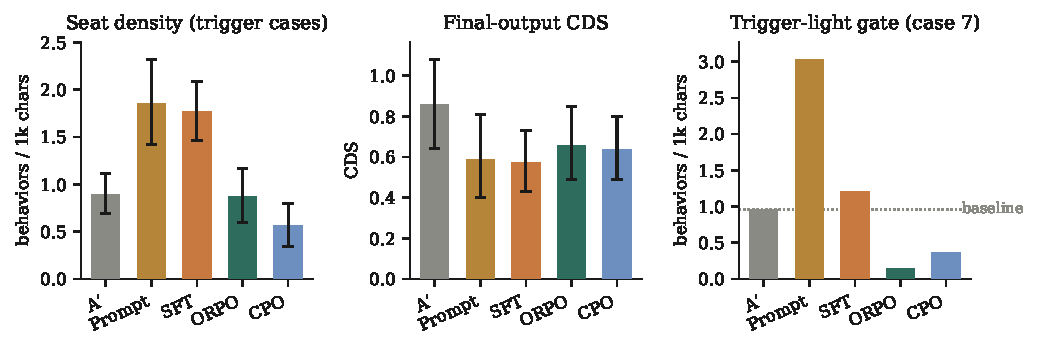
\includegraphics[width=\linewidth]{fig_triangle.pdf}
\caption{The installation triangle. Prompting and SFT install real seat-level
magnitude (left) that synthesis strips (center) and that fires on the
trigger-free control (right); preference optimization installs nothing and
suppresses the gate. Bars: means over $n=30$ run-level observations (6 trigger
cases $\times$ 5 seeds); whiskers: bootstrap 95\% CIs ($10^4$ resamples); gate
panel: $n=4$--$5$ per arm, dotted line = untrained baseline.}
\label{fig:triangle}
\end{figure}

\begin{table}[t]
\centering
\caption{Installation arms on the legal seat (cell-2 variance pass; $n=5$
seeds $\times$ 7 cases per arm, bootstrap 95\% CIs over run-level
observations). Bold marks CIs clear of baseline (seat) and the best value
per column.}
\label{tab:triangle}
\begin{tabular}{lccc}
\toprule
Arm & Seat density & Final-output CDS & Trigger-light gate \\
\midrule
$\text{A}'$ baseline & $0.89$ $[0.69,1.11]$ & $\mathbf{0.86}$ $[0.64,1.08]$ & $0.96$ \\
Prompting & $\mathbf{1.85}$ $[1.42,2.32]$ & $0.59$ $[0.40,0.81]$ & $3.03$ {\color{red!70!black}\ding{55}} \\
SFT-on-chosen & $\mathbf{1.77}$ $[1.46,2.09]$ & $0.58$ $[0.43,0.73]$ & $1.21$ {\color{red!70!black}\ding{55}} \\
ORPO & $0.87$ $[0.60,1.17]$ & $0.66$ $[0.49,0.85]$ & $\mathbf{0.15}$ {\color{green!45!black}\ding{51}} \\
\bottomrule
\end{tabular}
\end{table}

Prompting and SFT install real seat-level magnitude (CIs exclude baseline)---and both fail the gate, hedging on the trigger-free case (prompting despite its explicit ``do not force it'' clause). Both also lose their gains at the pipeline output: final CDS lands at or below the untrained baseline. ORPO installs no significant seat-level magnitude; its effect is qualitative---it is the only arm that \emph{suppresses} unwarranted hedging below baseline while leaving trigger-case behavior intact and imposing no content tax (rubric coverage identical to $\text{A}'$).

\textbf{The null is dose-invariant.} Retraining ORPO at $3.2\times$ dose (292 content-controlled pairs, epoch-matched to the 91-pair run) moved seat-level magnitude by zero: seat density $0.84$ $[0.58,1.11]$ vs.\ the 91-pair $0.85$ and baseline $0.84$, even though the larger set raised training-time preference accuracy from $0.48$ to $0.94$. More preference data was internalized but not emitted---strong evidence that ORPO's seat effect is not gradual installation of magnitude but a bounded suppression of unwarranted behavior. (The suppression itself weakened slightly with dose: the trigger-light gate rose from $0.15$ to $0.49$, still below baseline; more diverse pairs modestly broadened where the model deploys hedging.)

\textbf{The null generalizes across lineages; the suppression does not.} Pre-registered replications trained ORPO identically on two further seats. On the healthcare seat (Med42, already preference-aligned): no magnitude ($1.40$ $[1.15,1.68]$ vs.\ $\text{A}'$ $1.30$ $[1.07,1.54]$) and no responsiveness effect to detect---the untrained baseline already emits $0.00$ on the trigger-light case (dispatched in all runs); a pre-aligned model leaves no miscalibration slack to suppress. On the finance seat (Qwen-Open-Finance, SFT-only, Qwen-3): no magnitude ($1.32$ vs.\ $1.37$, CIs overlapping) and \emph{no suppression} (gate $0.81 \rightarrow 1.21$ under the pattern metric)---the replication prediction was falsified. The suppression is therefore conditional on base-model miscalibration and not guaranteed even then.

\textbf{The suppression is method-general; the selectivity is ORPO's.} A CPO arm \cite{cpoxu} on the identical legal pairs (only the objective changed) reproduces the gate suppression under both instruments ($0.37$ pattern / $0.45$ NLI-cutoff vs.\ $\text{A}'$'s $0.96$ / $1.06$)---but CPO also dampens \emph{warranted} trigger-case hedging ($0.89 \rightarrow 0.56$), where ORPO leaves it intact ($0.87$). Gate-to-trigger selectivity: $\text{A}'$ $1.08$, CPO $0.66$, ORPO $0.17$. Suppression is a property of reference-free preference optimization on these pairs; suppressing \emph{only where hedging is unwarranted} is, in our data, ORPO-specific.

\textbf{The null is family-general, not a cutoff artifact.} Because the
composite is dominated by one family, we re-tested each behavior on the seat
that owns it (App.~\ref{app:family}). ORPO moves none of them: finance
modeled-assumption $0.40$ $[0.31,0.49] \to 0.34$ $[0.24,0.45]$; healthcare
hedging $0.33 \to 0.26$; legal jurisdictional $0.14 \to 0.18$---all CIs
overlapping. Conversely, prompting and SFT install \emph{multiple} families,
including ones the seat previously emitted at zero (SFT on the legal seat:
modeled $0.00 \to 0.27$, hedging $0.02 \to 0.23$, alongside cutoff
$0.68 \to 1.21$), with one notable side effect---SFT \emph{suppressed}
jurisdictional distinguishing ($0.14 \to 0.02$) while installing the others.

\textbf{The null extends to the last writer.} If the register is merely where disposition happens to live, training the synthesizer itself should move it. It does not: ORPO on the Lead (same recipe, 88 dose-matched synthesis-level pairs, seats held at their untrained production versions) leaves the pipeline-mouth band unmoved --- final density $0.89$ $[0.67,1.11]$ vs.\ the conversion control's $1.03$ $[0.79,1.28]$, against a pre-registered threshold of $|\Delta|\ge 0.25$ with disjoint CIs. The control band also reproduces this writer's \S\ref{sec:register} register ($1.03$ vs.\ $1.24$), stable across cells. The trigger-light gate was already near-floor untrained ($0.15$), so no suppression is claimed --- the same no-slack situation as the pre-aligned seat. Weight-level training now fails at \emph{every} locus tested.

\textbf{Instrument validation.} Because these verdicts rest on measurement, we validated the instrument stack (\S\ref{app:instruments}): a calibrated NLI entailment scorer (chosen-vs-rejected AUC $0.929$ on the construction-labeled pair corpus) and blinded, order-swapped, evidence-grounded pairwise LLM judges \cite{llmjudge}. The magnitude nulls and healthcare zeros are instrument-robust (pattern + NLI); the legal suppression is three-instrument robust (pattern, NLI-cutoff $1.06 \rightarrow 0.35$, and $14/14$ decided judge pairs unanimous under both judges, sign-test $p=0.016$ each, no length bias); and the apparent finance \emph{reversal} ($0.81 \rightarrow 1.21$) appeared under the pattern metric only---NLI shows no increase on any family---and is retired as instrument artifact. The finance result stands as a non-replication (no suppression), not a worsening.

Two further details. First, prompting was tested at two loci: on the generalist single-shot (a $6\times$ final-output lift, $0.099 \rightarrow 0.589$, that failed the gate at $0.985$---its answer to the hybrid-work communication question opened a section ``Current State Snapshot (as of my training data)'' and closed with ``actual results may vary'': disclosure theater where nothing warranted disclosure) and on the seat (the table above). Second, content is unaffected by successful installation: rubric coverage is $12/36$ for both $\text{A}'$ and ORPO ($9/36$ for the original production seat)---no content tax. Gate cells use $n=4$--$5$ (the planner routes no specialists on the trigger-light case in some runs; routing variability is itself Ollama-runtime nondeterminism at temperature 0). Summary: \emph{prompting and exemplar training change what a model says, loudly and indiscriminately; preference training installs nothing---at best it removes miscalibrated hedging where the base model has it, ORPO selectively and CPO bluntly, and only the last writer decides what survives.}

\section{Result 3: the synthesizer register}
\label{sec:register}
Why do installed behaviors vanish? A pre-registered entanglement hypothesis---content-woven markers survive aggregation, detached boilerplate is stripped---was \textbf{refuted}: entangled share is flat across arms (baseline 56\%, prompting 61\%, ORPO 61\%, SFT 67\%---SFT's markers are the \emph{most} content-woven yet retain worst), retention splits by arm not position (baseline $1.08$, ORPO $0.96$ vs.\ prompting $0.49$, SFT $0.49$), and entanglement does not predict retention ($r=-0.10$ over 102 runs). Notably the refuted hypothesis and the overturned PRESERVE prediction (below) were both pre-registered---we report them as part of the record.

A 72-run ablation (2 input arms $\times$ 3 synthesizer models $\times$ PRESERVE instructions on/off $\times$ 6 cases) located the mechanism (Fig.~\ref{fig:register}, Table~\ref{tab:register}):

\begin{figure}[t]
\centering
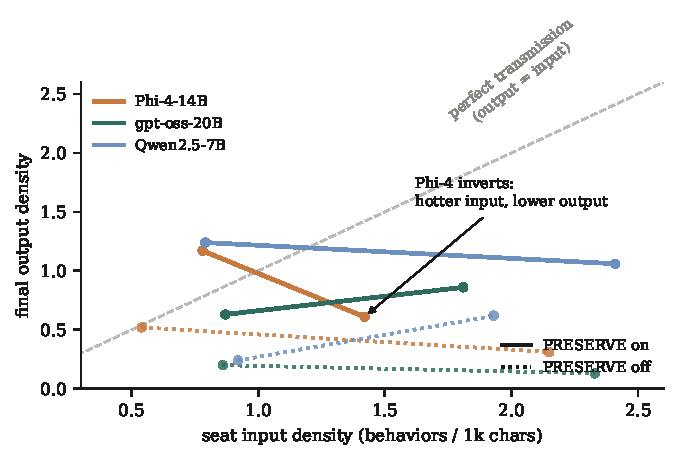
\includegraphics[width=0.72\linewidth]{fig_register.pdf}
\caption{The synthesizer register (72-run ablation). Every configuration sits
far below the perfect-transmission diagonal; slopes are nearly flat (input
density does not transmit) and Phi-4's is negative (over-dense input
\emph{inverts} output). Solid vs.\ dotted separates PRESERVE instructions
on/off---a $2$--$5\times$ gain on every Lead. Points: mean final-output density
over 6 cases per configuration.}
\label{fig:register}
\end{figure}

\begin{table}[t]
\centering
\caption{Final-output density by synthesizer $\times$ prompt $\times$ seat-input
arm (6 cases each; seat input densities in Fig.~\ref{fig:register}).}
\label{tab:register}
\begin{tabular}{lcccc}
\toprule
Synthesizer & \makecell{PRESERVE,\\base seat} & \makecell{PRESERVE,\\$2$--$3\times$ hot seat} & \makecell{no-PRESERVE,\\base} & \makecell{no-PRESERVE,\\hot} \\
\midrule
Phi-4-14B & $1.17$ & $0.61$ & $0.52$ & $0.31$ \\
gpt-oss-20B & $0.63$ & $0.86$ & $0.20$ & $0.13$ \\
Qwen2.5-7B & $1.24$ & $1.06$ & $0.24$ & $0.62$ \\
\bottomrule
\end{tabular}
\end{table}

Each synthesizer writes at its own characteristic density band regardless of input (registers are writer-specific \emph{under a fixed instruction set}---see \S\ref{sec:provenance} for the sense in which they are not); over-dense input does not transmit and can \emph{invert} output density (Phi-4: $1.17 \rightarrow 0.61$---over-correction, saturated hedging read as stylistic noise); and the PRESERVE instructions are a \textbf{gain control}, their removal collapsing output $2$--$5\times$ on every synthesizer (overturning our registered prediction that instructions would not matter). Mechanism: \emph{final disposition $\approx f(\text{register} \times \text{instructions})$, nearly independent of seat input. ORPO ``survives'' by staying inside the register; prompting and SFT ``strip'' by exceeding it.} The dose-invariance of \S\ref{sec:install} is the register's corollary: if the aggregator's band, not the seat's input, sets output disposition, then no amount of additional preference data at the seat can raise it---which is exactly what $3.2\times$ dose showed---and why the seat replications found no pipeline-level effect to transmit.

\begin{figure}[t]
\centering

\includegraphics[width=\linewidth]{fig_gain.pdf}
\caption{The register's two stress tests (96 runs). \emph{Left:} final-output
density rises with the number of PRESERVE clauses retained in the
synthesis prompt, on all three Leads (Spearman $\rho = +1.00 / +0.80 / +0.80$;
spans $3.3\times$ and $2.1\times$ for gpt-oss and Qwen). Phi-4's $k{=}2$ cell
(open marker) is anomalous---no other Lead bumps there and its within-cell
dispersion equals its between-level differences at $n{=}6$---and is reported as
probable noise. \emph{Right:} heating $h$ of 3 seats with the behavior-spec
override leaves pipeline-mouth density flat-to-declining ($\rho = -0.80$; CIs
overlap): seat disposition is not partially additive and then diluted, it does
not transmit. Points are means over 6 cases; whiskers bootstrap 95\% CIs.}
\label{fig:gain}
\end{figure}

\textbf{Stripping is family-dependent, and the surviving families are the
content-bearing ones.} Retention (final density $\div$ owner-seat density) at
baseline splits sharply: training-cutoff disclosure $0.69$ and hedging $0.76$
are stripped, whereas modeled-assumption flagging ($1.05$) and jurisdictional
distinguishing ($1.25$) pass through intact. A modeled number (``modeled at
\$8{,}000'') and a jurisdictional distinction carry substance the synthesizer
needs; a cutoff disclosure is meta-commentary it can drop without losing
content. This is a family-level analogue of the entanglement hypothesis that
\S\ref{sec:register} falsified at the \emph{arm} level: retention does not
split by arm or by marker position within a text, but it does split by whether
the behavior carries content. We report this as an observation from the
existing corpus, not a pre-registered test.

Two further ablations sharpen the mechanism (Fig.~\ref{fig:gain}). First, the
binary PRESERVE on/off contrast generalizes to a \emph{graded, monotone}
response: retaining $k \in \{0,1,2,3\}$ preservation clauses raises
final-output density on every Lead ($\rho=+1.00$, $+0.80$, $+0.80$)---instructions
are a measured gain control, not a switch. The relationship is a monotone
\emph{trend}, not strict monotonicity: only gpt-oss increases at every step,
while Qwen dips at $k{=}2$ ($0.999 \rightarrow 0.954$) and Phi-4 at $k{=}3$
($1.528 \rightarrow 0.675$); both departures are within the $n{=}6$ noise of
these cells. This trend is a property of the
\emph{composite}: pooled per-family, no single behavior is monotone in $k$
(cutoff $\rho=+0.40$, modeled $+0.60$, hedging $+0.40$, jurisdictional
$-0.80$), so instructions raise aggregate disposition without controlling any
individual behavior monotonically. Second, disposition is \emph{non-additive} in seat
input: applying the behavior-spec override to one, two, or all three seats
leaves the pipeline mouth flat ($\rho=-0.80$, spread $0.38$, overlapping
CIs)---closing the remaining alternative that seat disposition partially
accumulates and is diluted. Combined with the Lead-training null
(\S\ref{sec:install}), the mechanism statement finalizes as: \emph{final
disposition $\approx f(\text{register} \times \text{instructions})$, robust
to weight-level training at either locus; the accessible control surface is the
last writer's instructions.}

We then subjected the robustness clause to its strongest feasible test. The
Lead-training null used offline pairs with a density-shaped, response-level
reward---exactly the properties multiturn-aware reward training
\cite{collabllm} identifies as why behavioral installation fails. A
pre-registered follow-up corrected all three at once: syntheses sampled
\emph{on-policy} inside the running council ($n{=}6$ at $T{=}0.8$), scored at
the \emph{pipeline's mouth} with a \emph{calibration-shaped} reward
($+$CDS on trigger-heavy prompts, $-$density on trigger-light; 49 pairs
surviving a two-instrument directional gate), then ORPO under the identical
recipe. The register did not move: trained-vs-stock at $k{=}0$, $0.60$
$[0.41,0.82]$ vs.\ $0.56$ $[0.37,0.77]$; with instructions restored the
trained Lead sits at $0.95$, inside the stock band, and indistinguishable
from the density-rewarded arm ($0.89$)---so reward shape was not the earlier
null's binding constraint either. The instruction gain survives training at
full strength ($1.58\times$ vs.\ stock's $1.82\times$): the weights did not
absorb the instruction's role. (Best-of-$n$ distillation is a surrogate for
full on-policy RL, and the realized dose was 49 pairs; both caveats were
registered in advance.)

\section{Background: why disposition, not content}
The council was built to test whether small domain fine-tunes beat generalists on content. They do not: a single 20B open-weights MoE (gpt-oss-20B) outperforms the full council on rubric coverage ($42\%$ vs.\ $25\%$; $31\%$ after best-available specialist upgrades), and the council exhibited classic small-model failures (confabulated trial citations, repealed regulation treated as live). What specialists retained was disposition---the highest CDS of any configuration---which motivated the installation question this paper answers. We report this as motivating context, not a contribution.

\section{Where registers come from: the band is model-invariant}
\label{sec:provenance}
If model selection is the only lever that moves the register upward, what
makes one model's register higher than another's? We measured the
\emph{intrinsic} band: four models answering the seven cases under a minimal
neutral instruction, no council, no disposition instruction of any kind
(140 runs). The candidates span four base families and four alignment
lineages---Med42-8B (Llama-3, clinical SFT then DPO), BioMistral-7B (Mistral
v0.1, biomedical continued pretraining, no preference stage),
Mistral-7B-Instruct-v0.3 (generic instruct control in BioMistral's family),
and Qwen2.5-7B-Instruct.

Three of the four are indistinguishable: Med42 $0.15$ $[0.04,0.28]$,
Mistral-Instruct $0.14$ $[0.04,0.26]$, Qwen2.5 $0.14$ $[0.06,0.24]$, with
trigger-light gates of $0.00$ throughout. A fifth independent measurement
agrees---gpt-oss-20B single-shot under the same neutral prompt is $0.14$
(\S\ref{sec:arch})---so four models spanning four base architectures
(Llama-3, Mistral, Qwen2.5, and a MoE) share one band.

\textbf{The fourth candidate must be set aside, which costs us the
prediction.} BioMistral's published figure was $0.15$ $[0.00,0.41]$, but a
post-hoc integrity audit found that $26$ of its $30$ trigger runs are
degenerate: $208$--$463$ character fragments that terminate on a colon after
a setup sentence, with no analysis and no line breaks, under a
$8{,}192$-token cap the model never approached. Restricting to the four
substantive runs gives $0.29$ $[0.00,0.87]$---an interval too wide to
locate anything on a scale where every other model sits at $0.14$--$0.15$.
The direction of P8b.1 is unchanged under either reading (both intervals
overlap Med42's heavily), but the honest verdict is that the prediction is
\textbf{indeterminate rather than falsified}: our only
continued-pretraining-lineage arm failed to produce measurable output, so
the lineage contrast the cell was designed to make was never actually made.
We report the model-invariance result, which does not depend on it, and
withdraw the lineage claim. What survives is narrower and still useful: one
domain-SFT-plus-DPO model and three generically instruction-tuned models,
across four architectures, share a band to within $0.01$.

The between-synthesizer differences of \S\ref{sec:register} therefore
cannot be differences in baseline emission, since absent instructions every
model emits the same $\approx 0.14$. They are differences in
\emph{response} to the surrounding instructions. The register factor is
better read as a per-model \textbf{gain coefficient on instructions} than
as a characteristic emission level. For Qwen2.5 the decomposition is
measurable end to end: $0.14$ intrinsic, $0.56$ inside the council with
PRESERVE stripped, $1.03$ with the full block---roughly $4\times$ from the
scaffold and a further $1.8\times$ from the instructions, over a floor every
model shares. This also explains the two synthesizer-training nulls: a
LoRA-scale preference run has no purchase on \emph{how a model processes
instructions}, which is a far deeper property than a surface emission
tendency.

One practical corollary, and one caveat. Since the band is model-invariant,
a Lead should be selected for instruction \emph{responsiveness}, not for any
supposed intrinsic disposition: we found one candidate (OpenBioLLM-8B) that
ignores instructions in every message position and cannot emit the planner's
JSON, making it unusable as a last writer whatever its band---the control
surface operates through instructions, so following them is a prerequisite,
not a bonus. The registered caveat---that BioMistral's answers would be short and its
estimate coarse---turned out to understate the problem: the pre-run stability
screen sampled $248$--$555$ characters, but production runs ranged
$208$--$2{,}016$ and were bimodal within case, which the screen's three probes
could not reveal. A minimum-length guard on any density-style metric, and a
screen that samples the full case battery rather than three probes, would
have caught this before the runs.

\section{Which instruction does the work}
\label{sec:clause}
The gain curve of \S\ref{sec:register} varied the \emph{number} of PRESERVE
clauses, dropping them in a fixed order, so count was confounded with
identity. We isolated each clause against a true no-clause baseline on one
Lead (gpt-oss-20B, chosen for the widest gain range), 210 runs.

The block's gain is carried by a single clause, and it is not the one we
pre-registered. Against a no-clause baseline of $0.20$ $[0.14,0.26]$, the
numeric-framing clause alone reaches $0.64$ $[0.53,0.77]$---$126\%$ of the
full block's gain---while the caveats clause ($0.20$), the vocabulary clause
($0.18$), and the tension-acknowledgment clause ($0.19$) each land on the
baseline. Our prediction that caveats would carry the majority was
\textbf{falsified}; the tension clause, which the block's prose numbers
alongside the three PRESERVE clauses, carries nothing, settling that the
block is three working clauses and not four.

The per-family decomposition shows why, and rules out the alternative that
these instructions work by general priming. \emph{Every} clause lifts
exactly the family it names---numeric framing moves modeled-assumptions
$0.003 \rightarrow 0.499$, caveats moves cutoff $0.000 \rightarrow 0.035$,
vocabulary moves precision $0.000 \rightarrow 0.014$---and leaves the others
flat. The clauses are targeted behavior specifications. What differs is
headroom: only modeled-assumptions has enough mass under this synthesizer to
move the composite.

That makes the result Lead-specific in an important way. Across our ledger,
cutoff-disclosure dominates for Qwen2.5 ($0.554$) and production Phi-4
($0.909$) but is nearly absent for gpt-oss ($0.018$), which we selected
precisely for its dynamic range. The general statement the data supports is
therefore not ``write the numeric clause'' but: \emph{the block's gain is
carried by whichever clause targets the family the synthesizer already
produces in volume}; clauses aimed at families a given writer does not emit
are inert on the composite while still working on their own family. This
also explains the monotone count-curve of \S\ref{sec:register} without
appealing to count: adding clauses adds coverage, and the aggregate rises
whenever a newly added clause happens to match the writer's profile. The
clauses are mildly sub-additive (singles sum to $+0.41$ against the block's
$+0.35$; the numeric clause alone is numerically \emph{above} the full
block), consistent with that curve being compressive.

One property is unconditional: every arm, including each single clause,
holds the trigger-light gate at $0.00$ $[0.00,0.00]$. Conditionality is a
per-clause property, not an emergent feature of the assembled block---each
clause is an if-then over upstream evidence, so none of them fires when
nothing is flagged.

\section{Limitations}
\label{sec:limits}
Our five behavior families reduce to four in practice: vocabulary-precision is below detection ($\le 0.02$ density) on every seat and was also the worst-calibrated family for the NLI instrument (AUC $0.738$, Youden $J=0$), so two independent instruments fail it---either our cases do not provoke it or it is not detectable as a surface feature. The composite is cutoff-dominated \emph{for some synthesizers but not others} (Qwen2.5 $0.554$, Phi-4 $0.909$, but gpt-oss only $0.018$, where modeled-assumptions dominates instead), and the gain-curve monotonicity holds for the composite but not for any individual family. Pattern-based scoring has paraphrase blind spots and rewards concision; we mitigate with per-claim-normalized NLI scoring and pairwise LLM judges (\S\ref{app:instruments}), but the validation rests on inter-instrument convergence rather than a human-rated anchor---weaker on that axis than the human-validated certainty metric of \cite{certdist}---and two NLI hypothesis families calibrated degenerately (documented), and the judges' evidence-grounding gate rejected most pairs on dense numeric finance text. ORPO substitutes for DPO due to a memory defect in the only local DPO trainer available (documented); installation claims are scoped to reference-free preference optimization (ORPO, CPO). Suppression evidence concentrates on one weakly-aligned seat; trigger-light gate cells use $n=4$--$5$. The synthesizer-training null rests on one Lead (Qwen2.5-7B; a 14B Lead exceeded the training budget) at 88 pairs vs.\ the seat arms' 91, and its on-policy calibration-reward follow-up realized 49 pairs (its NLI directional gate was the binding filter) with best-of-$n$ distillation standing in for full RL; the gain-curve and additivity cells use $n=6$ per point without seed repeats, and two gain-curve cells depart from strict monotonicity---Phi-4's anomalous $k{=}2$ and Qwen's $k{=}2$ dip---both reported as probable noise at $n{=}6$; a seeded replication would settle them. A preference-data range of $91$--$292$ pairs (dose-invariant, but far larger scale untested), $n=5$ seeds. A corpus audit surfaced three provenance defects in the earliest (Result-2) arms, none of which changes a reported interval but all of which weaken those arms' internal consistency: in \texttt{local-council-\{repro,spec,sft,dpo\}} the five ``seeds'' per case are in fact one run from an earlier session plus four from a later one, with a directional $5$--$8\%$ length offset in three of the four arms; \texttt{local-council-dpo-v2} carries six runs on the trigger-light case against five elsewhere, slightly over-weighting it in unweighted means; and for $133$ runs the recorded model field holds a batch tag (\texttt{cell2-seed}, \texttt{dpo-experiment}) rather than a model identifier, so per-run model provenance is unrecoverable from the file for those runs. No seed field was ever written, which is what allowed the split sessions to go unnoticed; seven self-authored cases, and three local synthesizers $\le 20$B. The architecture comparison uses one model family (gpt-oss-20B) in every role and one instantiation of each design; debate and self-refine were implemented in their simplest standard forms and stronger variants may fare better. Frontier aggregators untested. The per-clause isolation (\S\ref{sec:clause}) ran on one synthesizer whose family profile we now know to be atypical; the Lead-dependence it implies is inferred from ledger profiles rather than tested directly, and a replication on a cutoff-dominant Lead is registered but not yet run. The intrinsic-band null covers four usable models at $\le 20$B under one neutral prompt (a fifth, BioMistral, produced degenerate output and was withdrawn post-hoc, taking the preference-vs-pretraining lineage contrast with it); a different neutral phrasing, or frontier-scale models, could separate them. All experiments ran on one consumer machine at \$0 API cost; we regard the reproducibility this buys as partial compensation for the scale it forgoes.

\section{Conclusion}
In multi-agent pipelines, epistemic disposition is not additive across stages: it is set by the last writer's register and that writer's instructions. Orchestration per se does not produce it---three specialists merged naively, or debating for two rounds, emit no more disposition than one model answering alone---and what the council buys is not magnitude but calibration: substantial disposition that stays silent when nothing warrants it, because its preservation instruction is conditional on real specialist signal. Upstream installation by prompting or exemplar tuning produces loud but indiscriminate behavior that the aggregator strips; preference optimization installs nothing at all---across three model lineages and a $3.2\times$ data dose---because the aggregator's register, not the seat, sets the ceiling. Its one dependable effect is subtractive: removing miscalibrated hedging where the base model has it, selectively under ORPO, bluntly under CPO, and on none of our seats reliably enough to treat as a design tool. The register itself withstands direct training of the synthesizer, and seat input is non-additive at the mouth---but the synthesis instructions form a monotone, $2$--$3\times$ gain control. In a multi-agent pipeline, the accessible control surface for epistemic disposition is not anyone's weights; it is the last writer's instructions. Builders who want calibrated pipelines should tune the synthesizer's instructions and choose the final model deliberately---and evaluate disposition at the pipeline's mouth, not the seat.

\paragraph{Reproducibility.} All code, prompts, 1{,}293 imported audited runs, pre-registrations, protocol amendments, verdicts (including refuted hypotheses), the pair datasets for all three seats, LoRA adapters, the NLI and judge instrument harnesses, and regeneration scripts: \url{https://github.com/srbobo/council-of-experts-research}.

\appendix
\section{Glossary}
\begin{description}[leftmargin=1em,style=nextline]
\item[Seat] one specialist model in the council, answering only its dispatched sub-question (e.g., Saul-7B $=$ the legal seat).
\item[Synthesizer / Lead] the model that receives all seat outputs plus the original question and compresses them into the final answer---the pipeline's last writer.
\item[Disposition] what a model chooses to emit independent of what it knows, operationalized as five behavior families: (1)~training-cutoff disclosure; (2)~modeled-assumption flagging; (3)~precise vocabulary distinctions; (4)~jurisdictional distinguishing; (5)~\textbf{hedging}---stated conditionality of a claim (``this may vary if\ldots''), \emph{not} refusal or vagueness. Family (3) proved below detection in our cases under two independent instruments; analyses report the four detectable families (App.~\ref{app:family}).
\item[Synthesis stripping] behavior density present at a seat's output but absent from the final output after synthesis.
\item[Synthesizer register] a Lead model's characteristic output disposition density---writer-specific and largely independent of seat input (\S6).
\item[Responsive vs.\ habitual] responsive behaviors appear only when domain triggers warrant them (trigger-light gate, case~7); habitual behaviors fire regardless.
\item[Alignment] post-pretraining procedures (SFT, RLHF, DPO/ORPO/CPO) shaping disposition, as distinct from the pretraining corpus, which shapes knowledge.
\end{description}

\section{Model selection}
Every selection cleared seven gates: (1)~GGUF availability on a mirror Ollama can pull; (2)~research-permissive license; (3)~ChatML-compatible or locally fixable chat template; (4)~recognized-lab provenance; (5)~distinct lineage per seat (four labs, three model families---a family-level training artifact cannot masquerade as a council effect); (6)~active maintenance; (7)~evidence of third-party use.

\textbf{Memory budget.} Sequential mode holds the Lead warm across all five phases, so peak $\approx M_{\text{lead}} + \max_{\text{seat}} M_{\text{seat}} + \text{KV} + \text{OS reserve} \le 32$\,GB; Metal's recommended working set on the test machine is 26.8\,GB. This bounds the Lead at $\le 14$B (Q4) and seats at $\le 8$B.

\textbf{Lead: Phi-4-14B} (MIT)---best reasoning-per-parameter at 14B for structured planner output; Qwen2.5-14B rejected on memory headroom, Llama-3.1-8B on synthesis capacity, 22--27B dense models on the Metal cap. The Lead is deliberately \emph{not} domain-tuned. \textbf{Healthcare: Llama3-Med42-8B}---the only 8B clinical fine-tune with a multi-stage \emph{preference-alignment} stage. \textbf{Legal: Saul-7B-Instruct-v1}---the only sub-13B continued pretrain (30B+ tokens) on multi-jurisdiction common-law text. \textbf{Finance: Qwen-Open-Finance-R-8B}---newest backbone of any seat (Qwen3), $>50\%$ finance corpus. \textbf{MoE comparator: gpt-oss-20B}---${\sim}3.6$B active parameters, reasoning-tuned, Apache-2.0; fits beside the Lead ($14+9=23$\,GB $< 26.8$\,GB), unlike Qwen3-30B-A3B (27\,GB) or Mixtral-8x7B (35\,GB).

\section{Metrics and estimation}
Let $B$ be the five behavior families and $P_b$ the regex pattern set for family $b$. For text $t$:
\begin{align*}
\text{Density}\quad & d(t) = \frac{1000}{|t|} \sum_{b\in B}\sum_{p\in P_b} |\text{matches}(p,t)|, \\
\text{Breadth}\quad & k(t) = \tfrac{1}{|B|}\,\big|\{\, b\in B : \exists p\in P_b,\ \text{matches}(p,t)\neq\varnothing \,\}\big|, \\
\text{CDS}\quad & \text{CDS}(t) = d(t)\cdot\sqrt{k(t)}, \\
\text{ALR}\quad & \text{ALR}_m = \bar d_{\text{council}}(m) \,/\, \bar d_{\text{single}}(\hat m), \\
\text{Retention}\quad & R = \text{clip}\big(d(\text{final})/d(\text{seat}),\, 0,\, 2\big).
\end{align*}
The square root in CDS softly penalizes narrow emission without letting one absent family zero the score (a geometric mean was rejected for exactly that failure); $\alpha=\tfrac12$ is a design choice, sensitivity unreported. Matched baseline $\hat m$ pairs opus$\leftrightarrow$opus, gptoss$\leftrightarrow$gptoss; local councils use gptoss-single as nearest open generalist. \emph{Worked example}: a 1{,}000-character answer with ``as of my training data (2024)'', ``modeled at \$8{,}000 assuming 60\% persistence'' ($\times 2$), and ``this may vary if the statute changes'' has $d=4.0$, $k=3/5$, $\text{CDS}=4.0\sqrt{0.6}\approx 3.10$. Uncertainty: percentile bootstrap over runs ($10^4$ resamples), 95\% intervals; $n=30$ per arm for trigger cases, $n=4$--$5$ for the trigger-light gate. Entanglement test (refuted): a marker sentence is \emph{entangled} if it also matches content signals (digits, \S, U.S.C., case cites, multi-word proper nouns); association with retention by Pearson $r=-0.10$ ($n=102$).

\section{Pair construction and training}
\textbf{Pair gates} (all must pass): chosen exhibits $\ge 2$ distinct behavior families; rejected exhibits $0$ across all five; length ratio $0.8 \le |\text{chosen}|/|\text{rejected}| \le 1.4$; content overlap $J(C(c),C(r)) \ge 0.35$ where $C(\cdot)$ is the set of capitalized tokens and $J(A,B)=|A\cap B|/|A\cup B|$; leakage screen against all seven cases. Yield: 200 prompts $\to$ 99 pairs (extended to 292 for the dose-response run).

\textbf{ORPO objective} \cite{orpo}: $\mathcal{L} = \mathcal{L}_{\text{SFT}} + \lambda\,\mathcal{L}_{\text{OR}}$ with $\mathcal{L}_{\text{OR}} = -\log\sigma\!\big(\log \tfrac{\text{odds}_\theta(y_w|x)}{\text{odds}_\theta(y_l|x)}\big)$ and $\text{odds}_\theta(y|x)=\tfrac{P_\theta(y|x)}{1-P_\theta(y|x)}$---a reference-free preference penalty added to the NLL of the chosen response.

\textbf{Configuration}: LoRA rank 8, scale 10, last 16 layers (10.5M trainable, ${\approx}0.145\%$); base loaded 4-bit; $\text{lr}=5\times10^{-6}$; batch 1, gradient accumulation 4; max sequence 1{,}792 (dataset $p_{100}=1{,}698$); 364 iterations (91-pair) / 1{,}056 (292-pair, epoch-matched); gradient checkpointing; seed 42. The SFT control is identical except SFT-mode on chosen-only data. Fused adapters follow the same fp16$\to$GGUF$\to$Q4\_K\_M conversion as the untrained control ($\text{A}'$), so the only delta between compared artifacts is the trained weights.

\section{Instrument validation}
\label{app:instruments}
\textbf{NLI scorer.} DeBERTa-v3-base-MNLI \cite{zeroshotnli} scores each sentence (Qwen-3 reasoning blocks stripped; per-claim normalization) against one frozen hypothesis per behavior family. Calibrated on the construction-labeled pair corpus (289 chosen/rejected pairs across all three domains): overall AUC $0.929$; per-family AUC $0.74$--$0.90$ with Youden thresholds frozen before verdict re-scoring. Two families calibrated degenerately (\emph{precise} non-discriminating; the \emph{hedging} hypothesis tracks substantive conditionality, which survives marker-stripping)---so gate arbitration uses the best-calibrated family (\emph{cutoff}, AUC $0.902$, $J=0.68$), and the registered all-family aggregate is reported as flawed.

\textbf{Pairwise judges.} Two local judges (gpt-oss-20B, Qwen2.5-7B) compare blinded $\text{A}' \times$ ORPO trigger-light seat outputs (cross-product pairing), each pair in both orderings at temperature 0; verdicts must quote evidence verbatim (non-matching quotes invalidate the call) and order-inconsistent verdicts count as ties. Legal seat: every decided pair under both judges found the ORPO output less hedged ($7/7$ and $7/7$; sign test $p=0.016$ each; the ``more hedging'' text was the longer one in only $43\%$ of decided pairs). Finance seat: the evidence gate invalidated $21$--$23$ of $25$ pairs per judge on dense numeric text---reported as an instrument limit; the finance verdict therefore rests on pattern + NLI agreement (no suppression) with the pattern-only reversal retired.

\textbf{Decision rule (pre-registered).} Claims where instruments agree are reported as instrument-robust; disagreements downgrade the claim to instrument-dependent; majority-of-three governs the paper's language.

\section{Per-family decomposition}
\label{app:family}
The composite metric sums five families that are unevenly distributed across
seats, so every headline claim was re-tested per family on the seat that owns
it (existing corpus; no additional inference).

\begin{table}[h]
\centering
\caption{Family ownership: untrained-baseline density (behaviors/1k chars) by
seat, and retention through synthesis (final $\div$ owner-seat density).}
\begin{tabular}{lcccc}
\toprule
Family & healthcare & legal & finance & retention \\
\midrule
training-cutoff & $0.85$ & $0.68$ & $0.51$ & $0.69$ \\
modeled-assumption & $0.00$ & $0.00$ & $\mathbf{0.25}$ & $1.05$ \\
hedging & $\mathbf{0.38}$ & $0.02$ & $0.33$ & $0.76$ \\
jurisdictional & $0.05$ & $\mathbf{0.14}$ & $0.13$ & $1.25$ \\
vocabulary-precision & $0.02$ & $0.00$ & $0.01$ & --- \\
\bottomrule
\end{tabular}
\end{table}

Summary of the decomposition: (i)~the ORPO magnitude null holds for every
family on its owner seat and for all four families in the Lead-training arm;
(ii)~prompting and SFT install several families at once, including ones
previously at zero, while SFT suppresses jurisdictional distinguishing;
(iii)~stripping is family-dependent (content-bearing families survive);
(iv)~the gain-curve trend is a composite property and is a rank trend rather than strict monotonicity; (v)~non-additivity holds
for the two families with sufficient signal (cutoff $\rho=-0.80$, hedging
$\rho=-1.00$). The decomposition script is versioned with the code.

\section{Key prompts (verbatim excerpts)}
\label{app:prompts}
Full text of every prompt is versioned in the repository; the two most
load-bearing are excerpted here.

\textbf{Pairwise judge prompt} (Cell 7b; \texttt{\{text\_a\}}/\texttt{\{text\_b\}}
are the blinded seat outputs):
\begin{quote}\small\ttfamily
You are auditing two analyst responses for UNWARRANTED epistemic hedging.
[\ldots] This question involves NO regulatory, legal, medical, or financial
uncertainty. [\ldots] UNWARRANTED EPISTEMIC HEDGING means any of the following,
when nothing in the question calls for it: (1) Training-cutoff or
knowledge-limit disclosures (``as of my training data\ldots'', ``verify current
guidance\ldots'') (2) Labeling ordinary statements as assumptions or models
(``assuming that\ldots'', ``modeled at\ldots'') (3) Hedged conditionality on
claims that need none (``this may vary if\ldots'') (4) Disclaimers, ``actual
results may vary'' boilerplate, or accuracy caveats. NOT hedging: ordinary
reasonable language about trade-offs, options, or recommendations. Judging
substance or quality is NOT your task. [\ldots] Which response contains MORE
unwarranted epistemic hedging? Reply with ONLY this JSON:
\{``verdict'': ``A''\,$|$\,``B''\,$|$\,``TIE'', ``evidence\_a'': [verbatim
quotes], ``evidence\_b'': [\ldots]\}. Quote every hedging instance verbatim.
\end{quote}

\textbf{Pair-generation rewrite templates} (Appendix~D pairs; both operate on
the same base answer):
\begin{quote}\small\ttfamily
REWRITE\_ADD: Rewrite the analysis below so that it additionally exhibits
these professional-discipline behaviors WHEREVER RELEVANT---without changing
its substantive content, structure, or approximate length: (1) training-cutoff
disclosure \ldots (2) modeled-assumption flagging \ldots (3) precise
vocabulary \ldots (4) jurisdictional distinguishing \ldots (5) hedged
uncertainty \ldots Do NOT add new substantive claims. Do NOT lengthen by more
than ${\sim}15\%$.

REWRITE\_STRIP: Rewrite the analysis below to REMOVE all of the following,
without changing its substantive content, structure, or approximate length:
any mention of training cutoffs \ldots any labeling of numbers as assumptions
\ldots any explicit distinguishing of near-synonym terms \ldots any
jurisdiction-by-jurisdiction separation language \ldots any hedging about what
might vary. State everything with plain confidence.
\end{quote}

\begin{thebibliography}{99}
\small
\bibitem{du2023} Du, Y.\ et al.\ Improving Factuality and Reasoning in Language Models through Multiagent Debate. arXiv:2305.14325 (2023).
\bibitem{moa2024} Wang, J.\ et al.\ Mixture-of-Agents Enhances Large Language Model Capabilities. arXiv:2406.04692 (2024).
\bibitem{medagents} Tang, X.\ et al.\ MedAgents: LLMs as Collaborators for Zero-shot Medical Reasoning. arXiv:2311.10537 (2023).
\bibitem{mdagents} Kim, Y.\ et al.\ MDAgents: An Adaptive Collaboration of LLMs for Medical Decision-Making. arXiv:2404.15155 (NeurIPS 2024).
\bibitem{tian2025} Tian, A.X.\ et al.\ Beyond the Strongest LLM: Multi-Turn Multi-Agent Orchestration vs.\ Single LLMs on Benchmarks. arXiv:2509.23537 (2025).
\bibitem{masorchestra} Ke, Z.\ et al.\ MAS-Orchestra: Understanding and Improving Multi-Agent Reasoning. arXiv:2601.14652 (2026).
\bibitem{parallelsynth} Towards Direct Latent-Space Synthesis for Parallel Branches in LLM-Agent Workflows. arXiv:2606.14672 (2026).
\bibitem{trident} Hui, Z., Dong, Y.R., Shareghi, E., Collier, N. TRIDENT: Benchmarking LLM Safety in Finance, Medicine, and Law. arXiv:2507.21134 (2025).
\bibitem{medftrag} Buskila, A.A. Domain Fine-Tuning vs.\ Retrieval-Augmented Generation for Medical Multiple-Choice Question Answering: A Controlled Comparison at the 4B-Parameter Scale. arXiv:2604.23801 (2026).
\bibitem{lin2022} Lin, S., Hilton, J., Evans, O. Teaching Models to Express Their Uncertainty in Words. arXiv:2205.14334 (2022).
\bibitem{mielke2022} Mielke, S.J.\ et al.\ Reducing Conversational Agents' Overconfidence through Linguistic Calibration. TACL (2022).
\bibitem{kadavath2022} Kadavath, S.\ et al.\ Language Models (Mostly) Know What They Know. arXiv:2207.05221 (2022).
\bibitem{rtuning} Zhang, H.\ et al.\ R-Tuning: Instructing LLMs to Say `I Don't Know'. arXiv:2311.09677 (NAACL 2024).
\bibitem{icalm} Zong, H.\ et al.\ I-CALM: Incentivizing Confidence-Aware Abstention. arXiv:2604.03904 (2026).
\bibitem{bas} Wu, S.\ et al.\ BAS: A Decision-Theoretic Approach to Evaluating LLM Confidence. arXiv:2604.03216 (2026).
\bibitem{markerfaith} Can LLMs Use Linguistic Uncertainty Markers to Reliably Reflect Intrinsic Confidence? arXiv:2605.28778 (2026).
\bibitem{rhetmiscal} Saying More Than They Know: Quantifying Epistemic-Rhetorical Miscalibration in LLMs. arXiv:2604.19768 (2026).
\bibitem{markerrel} Revisiting Epistemic Markers in Confidence Estimation. arXiv:2505.24778 (2026).
\bibitem{dpo} Rafailov, R.\ et al.\ Direct Preference Optimization. arXiv:2305.18290 (NeurIPS 2023).
\bibitem{orpo} Hong, J., Lee, N., Thorne, J. ORPO: Monolithic Preference Optimization without Reference Model. arXiv:2403.07691 (EMNLP 2024).
\bibitem{lengthbias} Park, R.\ et al.\ Disentangling Length from Quality in DPO. arXiv:2403.19159 (2024).
\bibitem{sweetspot} Finding the Sweet Spot: Preference Data Construction for Scaling Preference Optimization. arXiv:2502.16825 (2025).
\bibitem{air} AIR: A Systematic Analysis of Annotations, Instructions, and Response Pairs in Preference Datasets. arXiv:2504.03612 (2025).
\bibitem{certdist} Belem, C.G., Wu, S., Yao, H., Steyvers, M., Singh, S., Smyth, P. From `May' to `Is': Certainty Distortion in Language Model Rewriting. arXiv:2606.07951 (2026).
\bibitem{possdef} Possible or Definite? A Benchmark for Evaluating Diagnostic Uncertainty Preservation in Clinical Text. arXiv:2606.18471 (2026).
\bibitem{laundering} Confidence Laundering in Agent Systems: Why Uncertainty Needs a Latent Carrier. arXiv:2606.20662 (2026).
\bibitem{uprop} Da, J.\ et al.\ UProp: Investigating the Uncertainty Propagation of LLMs in Multi-Step Agentic Decision-Making. arXiv:2506.17419 (2025).
\bibitem{cpoxu} Xu, H.\ et al.\ Contrastive Preference Optimization: Pushing the Boundaries of LLM Performance in Machine Translation. arXiv:2401.08417 (2024).
\bibitem{zeroshotnli} Yin, W., Hay, J., Roth, D. Benchmarking Zero-shot Text Classification: Datasets, Evaluation and Entailment Approach. arXiv:1909.00161 (EMNLP 2019). Model: MoritzLaurer/DeBERTa-v3-base-mnli-fever-anli.
\bibitem{llmjudge} Zheng, L.\ et al.\ Judging LLM-as-a-Judge with MT-Bench and Chatbot Arena. arXiv:2306.05685 (NeurIPS 2023).
\bibitem{collabllm} Wu, S.\ et al.\ CollabLLM: From Passive Responders to Active Collaborators. arXiv:2502.00640 (2025).
\bibitem{voicerev} Voice Under Revision: Large Language Models and the Normalization of Personal Narrative. arXiv:2604.22142 (2026).
\bibitem{singleagent} Tran, D., Kiela, D. Single-Agent LLMs Outperform Multi-Agent Systems on Multi-Hop Reasoning Under Equal Thinking Token Budgets. arXiv:2604.02460 (2026).
\bibitem{stepback} Zheng, H.S.\ et al.\ Take a Step Back: Evoking Reasoning via Abstraction. arXiv:2310.06117 (ICLR 2024).
\end{thebibliography}

\end{document}
